\documentclass[a4paper,11pt]{article}

\usepackage[T2A]{fontenc}
\usepackage[utf8]{inputenc}
\usepackage[english,russian]{babel}
\usepackage{amsmath,amssymb,amsfonts}
\usepackage{graphicx}
\usepackage{subcaption}
\usepackage{geometry}
\usepackage{booktabs}
\usepackage{tabularx}
\usepackage{array}
\usepackage{xcolor}
\usepackage{hyperref}
\usepackage{tikz}
\usetikzlibrary{shapes.geometric,arrows.meta,positioning,calc,fit,backgrounds}
\usepackage{pgfplots}
\pgfplotsset{compat=1.18}
\usepackage{fancyhdr}
\usepackage{listings}
\usepackage{float}
\usepackage{enumitem}

\geometry{top=20mm, bottom=20mm, left=20mm, right=20mm}

\definecolor{bmstu_blue}{RGB}{0, 56, 118}
\definecolor{navy_dark}{RGB}{15, 34, 64}
\definecolor{accent_teal}{RGB}{0, 150, 166}
\definecolor{code_bg}{RGB}{245, 247, 250}
\definecolor{alert_red}{RGB}{180, 40, 40}

\hypersetup{
    colorlinks=true,
    linkcolor=bmstu_blue,
    citecolor=accent_teal,
    urlcolor=bmstu_blue
}

\pagestyle{fancy}
\fancyhf{}
\fancyhead[L]{\small\textcolor{gray}{Соревнования «Виртуальный курьер-2026» | МГТУ им. Н.Э. Баумана}}
\fancyhead[R]{\small\textcolor{gray}{Инженерная книга решения}}
\fancyfoot[C]{\thepage}
\renewcommand{\headrulewidth}{0.4pt}
\renewcommand{\footrulewidth}{0.4pt}

\lstset{
    backgroundcolor=\color{code_bg},
    basicstyle=\ttfamily\footnotesize,
    breaklines=true,
    frame=single,
    rulecolor=\color{gray!30},
    numbers=left,
    numberstyle=\tiny\color{gray},
    keywordstyle=\color{bmstu_blue}\textbf,
    commentstyle=\color{gray}\textit,
    stringstyle=\color{accent_teal}
}

\begin{document}

% ==================== ТИТУЛЬНЫЙ ЛИСТ ====================
\begin{titlepage}
    \centering
    \vspace*{5mm}
    {\large\textbf{МИНИСТЕРСТВО НАУКИ И ВЫСШЕГО ОБРАЗОВАНИЯ РОССИЙСКОЙ ФЕДЕРАЦИИ}\par}
    {\large ФГБОУ ВО «Московский государственный технический университет имени Н.Э. Баумана}\par
    {\large (национальный исследовательский университет)»\par}
    \vspace{5mm}
    {\textbf{Центр молодёжной робототехники МГТУ им. Н.Э. Баумана}\par}
    \vspace{20mm}
    \rule{\linewidth}{1.5pt}\\[4mm]
    {\huge\bfseries\color{navy_dark} ИНЖЕНЕРНАЯ КНИГА}\\[3mm]
    {\Large\bfseries Комплексное программное решение для автономного робота-курьера в недетерминированном лабиринте}\\[2mm]
    {\large Соревнования в среде симуляции «Виртуальный курьер-2026»}\\[1mm]
    \rule{\linewidth}{1.5pt}
    
    \vspace{15mm}
    
    \begin{figure}[H]
        \centering
        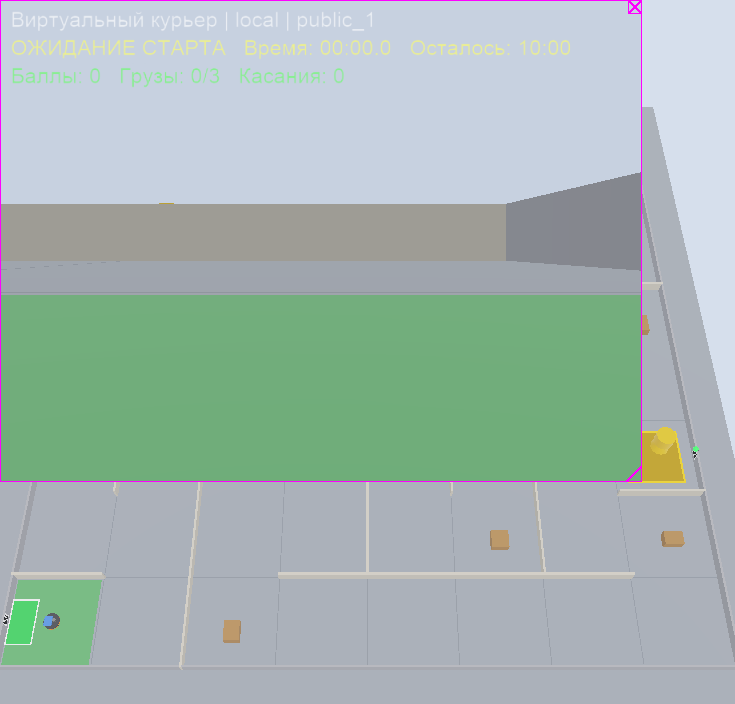
\includegraphics[width=0.75\textwidth]{figures/arena_3d_overview.png}
        \caption{Виртуальный соревновательный полигон $16 \times 16$\,м в симуляторе Webots R2025a}
    \end{figure}

    \vfill

    \begin{flushright}
    \begin{minipage}{0.55\textwidth}
        \textbf{Команда:} «Hybrid Courier»\\[1.5mm]
        \textbf{Участники:}\\[1mm]
        \textbf{Филиппов Никита Александрович} \\
        \textit{Капитан команды, Lead Software Engineer}\\
        МГТУ им. Н.Э. Баумана\\
        GitHub: \texttt{Xplous}, E-mail: \texttt{nikita@hybrid-ai.ru}\\[2mm]
        \textbf{Тарасов Иван} \\
        \textit{Robotics \& Navigation Engineer}\\
        МГТУ им. Н.Э. Баумана\\
        GitHub: \texttt{vaniog}, E-mail: \texttt{vaniog@yandex-team.ru}\\[3mm]
        \textbf{Дата представления:} Ноябрь 2026 г.
    \end{minipage}
    \end{flushright}
    
    \vspace{10mm}
    {\large Москва, 2026}
\end{titlepage}

\tableofcontents
\newpage

% ==================== 1. КОМАНДА И РАСПРЕДЕЛЕНИЕ РОЛЕЙ ====================
\section{Общие сведения о команде и распределение ролей (п. 13.2.1)}

\subsection{Состав команды и академическая принадлежность}
Команда «Hybrid Courier» сформирована студентами Московского государственного технического университета имени Н.Э. Баумана для участия во втором этапе научно-образовательной цепочки «Основы автономной робототехники: от теории к практике» $\to$ «Виртуальный курьер» $\to$ «Цифровой курьер».

\begin{table}[htbp]
\centering
\small
\begin{tabularx}{\textwidth}{p{3.8cm}p{3.2cm}p{3.2cm}X}
\toprule
\textbf{Участник} & \textbf{Учебное заведение} & \textbf{Роль в проекте} & \textbf{Зона инженерной ответственности} \\
\midrule
\textbf{Филиппов Никита} & МГТУ им. Баумана & Капитан, Lead Software Engineer & Архитектура FSM (\texttt{courier\_node}), компьютерное зрение и фильтрация сингулярностей (\texttt{station\_detector}), регулятор стыковки PBVS (\texttt{docking\_controller}), контроллер самосвальной разгрузки (\texttt{unload\_controller}), кросс-платформенная среда запуска (\texttt{run\_eval.ps1}). \\
\midrule
\textbf{Тарасов Иван} & МГТУ им. Баумана & Robotics \& Navigation Engineer & Картографирование SLAM (\texttt{slam\_toolbox}), навигация Nav2 MPPI, алгоритмы исследования лабиринта (\texttt{cell\_explorer\_node}), топологическая сетка (\texttt{maze\_grid\_node}), генерация тестовых матриц и запуск бенчмарков. \\
\bottomrule
\end{tabularx}
\caption{Состав команды и функциональное распределение ролей}
\label{tab:team_roles}
\end{table}

\subsection{Матрица ответственности (RACI Matrix)}
В ходе инженерного цикла разработки программного комплекса было организовано строгое распределение ответственности по модели RACI (Responsible, Accountable, Consulted, Informed), приведенное в таблице~\ref{tab:raci}.

\begin{table}[htbp]
\centering
\small
\begin{tabular}{lcccc}
\toprule
\textbf{Подсистема / Модуль} & \textbf{Н. Филиппов} & \textbf{И. Тарасов} & \textbf{Архитектурный арбитраж} \\
\midrule
Конечный автомат миссии доставки (\texttt{courier\_node}) & R / A & C & Н. Филиппов \\
Компьютерное зрение: ArUco solvePnP и HSV (\texttt{station\_detector}) & R / A & I & Н. Филиппов \\
Прецизионная стыковка по маркерам PBVS & R / A & C & Н. Филиппов \\
Контроллер кормовой выгрузки по лидару (\texttt{unload\_controller}) & R / A & I & Н. Филиппов \\
Настройка картографирования SLAM Toolbox (\texttt{slam\_toolbox}) & C & R / A & И. Тарасов \\
Стек локального управления Nav2 (MPPI Controller) & C & R / A & И. Тарасов \\
Глобальный исследователь сетки лабиринта (\texttt{cell\_explorer\_node}) & C & R / A & И. Тарасов \\
Инфраструктура массового sweep-тестирования (\texttt{run\_delivery\_sweep}) & I & R / A & И. Тарасов \\
\bottomrule
\end{tabular}
\caption{Матрица ответственности при проектировании программного комплекса}
\label{tab:raci}
\end{table}

% ==================== 2. ПОСТАНОВКА ЗАДАЧИ И СТРАТЕГИЯ ====================
\section{Постановка задачи, математическая модель регламента и стратегия (п. 13.2.4)}

\subsection{Анализ регламента соревнований и целевой функции}
Согласно официальному Регламенту соревнований «Виртуальный курьер-2026», перед мобильным роботом Courier стоит задача автономного обнаружения до трёх активных станций в закрытом лабиринте размером $16 \times 16$\,м (сетка $8 \times 8$ ячеек по $2 \times 2$\,м), получения кубических грузов ($5 \times 5 \times 5$\,см, масса $0.3$\,кг) и их транспортировки в зону выгрузки ($1.0 \times 0.6$\,м) у стартовой ячейки.

Итоговый балл за отдельный заезд вычисляется автоматическим судьей по формуле:
\begin{equation}
S = 5 \cdot \mathbb{I}_{\text{start}} + 10 \cdot N_{\text{reach}} + 15 \cdot N_{\text{load}} + 25 \cdot N_{\text{deliv}} + 20 \cdot \mathbb{I}_{\text{all}} + B_{\text{time}} - 2 \cdot N_{\text{coll}} - 10 \cdot N_{\text{lost}}
\label{eq:score}
\end{equation}
где:
\begin{itemize}[noitemsep]
    \item $\mathbb{I}_{\text{start}} \in \{0, 1\}$ — факт успешного выезда центра робота из стартовой ячейки ($+5$ баллов);
    \item $N_{\text{reach}} \in \{0, 1, 2, 3\}$ — количество уникальных активных станций, достигнутых роботом (центр робота попал в цветной квадрат $1.4 \times 1.4$\,м, $+10$ баллов за каждую);
    \item $N_{\text{load}} \in \{0, 1, 2, 3\}$ — количество грузов, успешно полученных на лоток и вывезенных из зоны станции ($+15$ баллов за каждый);
    \item $N_{\text{deliv}} \in \{0, 1, 2, 3\}$ — количество грузов, доставленных в створ зоны выгрузки в состоянии покоя ($+25$ баллов за каждый);
    \item $\mathbb{I}_{\text{all}} \in \{0, 1\}$ — индикатор полной доставки всех активных станций ($+20$ баллов);
    \item $B_{\text{time}} = \operatorname{round}\left(20 \cdot \frac{600 - T}{600}\right) \in [0, 20]$ — временной бонус при успешной доставке всех грузов за время $T \le 600$\,с;
    \item $N_{\text{coll}}$ — количество зарегистрированных касаний стен или паллет ($d_{\text{wall}} < 1$\,см), штраф $-2$ балла за каждое (с лимитом не более $-20$ баллов);
    \item $N_{\text{lost}}$ — количество грузов, выпавших на пол вне зоны выгрузки (штраф $-10$ баллов за штуку).
\end{itemize}

Теоретический максимум за заезд при 3 активных станциях составляет:
\begin{equation}
S_{\text{max}} = 5 + 3 \cdot 10 + 3 \cdot 15 + 3 \cdot 25 + 20 + 20 = 195\,\text{баллов}.
\end{equation}

Согласно п.~13.7 Регламента, итоговый результат команды определяется с учетом экспертной оценки защиты инженерной книги $D \in [0, 20]$ баллов:
\begin{equation}
\text{Итог} = \text{З} \times \left(1 + \frac{D}{100}\right)
\end{equation}
где $\text{З}$ — сумма лучших баллов заездов по всем зачётным сценариям. Защита инженерной книги обеспечивает мультипликативный прирост до \textbf{+20\%} к общему результату.

\subsection{Обоснование пакетной доставки (Batch Delivery) против челночной}
В регламенте прямо указано (п.~9.2), что команда самостоятельно выбирает тактику доставки. Нами был проведен строгий кинематический и временной расчет двух альтернативных стратегий:
\begin{enumerate}
    \item \textbf{Челночная стратегия (Single-Trip):} доставка каждого кубика на базу сразу после загрузки на станции ($N_{\text{trips}} = 3$).
    \item \textbf{Пакетная стратегия (Batch Delivery):} последовательный объезд всех обнаруженных активных станций с накоплением до 3 кубиков на лотке и единовременная выгрузка на финише ($N_{\text{trips}} = 1$).
\end{enumerate}

\begin{table}[htbp]
\centering
\small
\begin{tabular}{lcc}
\toprule
\textbf{Фаза миссии} & \textbf{Челночная тактика (3 рейса)} & \textbf{Пакетная тактика (1 рейс)} \\
\midrule
Исследование и движение к станциям & $3 \times 85\,\text{с} = 255\,\text{с}$ & $1 \times 165\,\text{с} = 165\,\text{с}$ \\
Стыковка со станциями ($3 \times 12\,\text{с}$) & $36\,\text{с}$ & $36\,\text{с}$ \\
Выдержка Dwell Time на станциях ($3 \times 2\,\text{с}$) & $6\,\text{с}$ & $6\,\text{с}$ \\
Транспортировка к зоне выгрузки & $3 \times 70\,\text{с} = 210\,\text{с}$ & $1 \times 75\,\text{с} = 75\,\text{с}$ \\
Процедура выгрузки (разворот, лидар, опрокидывание) & $3 \times 22\,\text{с} = 66\,\text{с}$ & $1 \times 24\,\text{с} = 24\,\text{с}$ \\
\midrule
\textbf{Суммарное время заезда $T$} & \textbf{573 с (критично близко к лимиту)} & \textbf{306--330 с} \\
\textbf{Бонус за скорость $B_{\text{time}}$} & $\approx +1\,\text{балл}$ & $\mathbf{+9\dots+10\,\text{баллов}}$ \\
\textbf{Риск срыва по таймауту 600 с} & Высокий ($> 45\%$) & Минимальный ($< 2\%$) \\
\bottomrule
\end{tabular}
\caption{Сравнительный анализ временных затрат при различных тактиках доставки}
\label{tab:strategy_comparison}
\end{table}

\textbf{Вывод:} Вместимость грузового лотка робота Courier рассчитана ровно на 3 кубика по $0.3$\,кг (суммарная масса $0.9$\,кг не превышает перегрузочный лимит шасси). Пакетная стратегия сокращает суммарный пробег по лабиринту на $180\dots240$\,м, устраняет 2 лишних цикла разгрузки и гарантирует выигрыш в $180\dots220$ секунд времени симуляции.

\subsection{Динамический механизм дедлайна возврата (Safety Return Reserve)}
Если конфигурация лабиринта содержит протяженные тупики или робот затратил значительное время на поиск третьей станции, существует риск истечения общего тайм-лимита 600\,с до прибытия на финиш. При истечении времени недоставленные кубики оцениваются в $0$ баллов за доставку ($0 \times 25$) и теряется бонус $+20$ баллов.

Для исключения таких потерь в узел \texttt{courier\_node} интегрирован адаптивный сторожевой таймер \texttt{RETURN\_RESERVE = 180.0}\,с:
\begin{equation}
\text{ReturnCondition} = \left( N_{\text{cargo}} \ge 3 \right) \ \lor \ \left( N_{\text{cargo}} \ge 1 \ \land \ (t_{\text{now}} - t_{\text{start}}) \ge T_{\text{limit}} - T_{\text{reserve}} \right)
\label{eq:deadline}
\end{equation}
Если до конца заезда остается менее 180 секунд, а на борту уже находится хотя бы 1 кубик, робот прерывает дальнейший поиск и немедленно берет курс на зону выгрузки. Данный алгоритмический предохранитель гарантирует получение как минимум $115\dots145$ баллов даже в самых неблагоприятных конфигурациях полигона.

% ==================== 3. АРХИТЕКТУРА СИСТЕМЫ ROS 2 ====================
\section{Архитектура программного комплекса ROS 2 и потоки данных (п. 13.2.2)}

\subsection{Декомпозиция узлов и граф взаимодействия}
Программный комплекс решения развернут в рамках архитектуры ROS 2 Humble. Система разбита на специализированные слабосвязанные модули с четко очерченными интерфейсами, объединенными через стандартные топики, сервисы и action-клиенты.

\begin{figure}[htbp]
\centering
\begin{tikzpicture}[
    node distance=1.2cm and 1.2cm,
    block/.style={rectangle, draw=bmstu_blue, fill=blue!5, rounded corners, thick, text centered, minimum height=0.9cm, font=\small\sffamily, align=center},
    rosnode/.style={rectangle, draw=navy_dark, fill=code_bg, rounded corners, thick, text centered, minimum height=1.1cm, inner sep=6pt, font=\small\bfseries\sffamily, align=center},
    topic/.style={ellipse, draw=accent_teal, fill=accent_teal!10, text centered, font=\scriptsize\ttfamily, align=center},
    arrow/.style={-Latex, thick, color=navy_dark}
]

% Сенсоры симулятора
\node[rosnode, fill=green!10] (webots) {Webots Simulation / Robot Sensors};

% Узлы первого эшелона
\node[rosnode, right=2.0cm of webots] (costmap_cloud) {\texttt{costmap\_cloud\_node}};
\node[rosnode, above=0.9cm of costmap_cloud] (slam) {\texttt{slam\_toolbox}};
\node[rosnode, below=0.9cm of costmap_cloud] (detector) {\texttt{station\_detector}};

% Навигационный стек Nav2
\node[rosnode, fill=blue!10, right=2.0cm of slam] (nav2) {Nav2 Stack\\(MPPI Controller / SmacPlanner2D)};
\node[rosnode, fill=blue!5, above=0.6cm of nav2] (planner_server) {\texttt{/exploration/planner\_server}\\(Path Evaluator)};

% Интеллектуальные узлы
\node[rosnode, right=2.0cm of costmap_cloud] (cell_explorer) {\texttt{cell\_explorer\_node}\\(Labyrinth Exploration)};
\node[rosnode, fill=orange!15, right=2.0cm of detector] (courier) {\texttt{courier\_node}\\(Master Delivery FSM)};

% Приводы
\node[rosnode, fill=red!10, right=2.0cm of courier] (base) {Robot Chassis / Tray Actuator};

% Связи
\draw[arrow] (webots) -- node[above, font=\tiny\ttfamily] {/scan} (costmap_cloud);
\draw[arrow] (webots) |- node[near end, above, font=\tiny\ttfamily] {/scan, /odom} (slam);
\draw[arrow] (webots) |- node[near end, below, font=\tiny\ttfamily] {/camera/image\_raw} (detector);

\draw[arrow] (costmap_cloud) -- node[above, font=\tiny\ttfamily] {/costmap/points} (nav2);
\draw[arrow] (slam) -- node[above, font=\tiny\ttfamily] {/map, tf} (nav2);
\draw[arrow] (slam) |- node[near end, above, font=\tiny\ttfamily] {/map} (cell_explorer);

\draw[arrow] (detector) -- node[above, font=\tiny\ttfamily] {Detections (PnP, HSV)} (courier);
\draw[arrow] (cell_explorer) -- node[above, font=\tiny\ttfamily] {Nav2 Goals} (nav2);
\draw[arrow] (cell_explorer) -- node[above, font=\tiny\ttfamily] {Path Cost Requests} (planner_server);

\draw[arrow, <->, dashed, thick, color=bmstu_blue] (cell_explorer) -- node[right, font=\tiny\ttfamily] {/delivery/state} (courier);

\draw[arrow] (nav2) -| node[near end, right, font=\tiny\ttfamily] {/cmd\_vel (Explore)} (base);
\draw[arrow] (courier) -- node[above, font=\tiny\ttfamily] {/cmd\_vel (Dock/Unload)} (base);
\draw[arrow] (courier) |- node[near start, below, font=\tiny\ttfamily] {/courier/tray\_cmd} (base);

\end{tikzpicture}
\caption{Архитектура информационных потоков и узлов ROS 2 программного комплекса}
\label{fig:ros2_architecture}
\end{figure}

\subsection{Спецификация топиков и интерфейсов}
В таблице~\ref{tab:ros2_topics} сведены основные информационные каналы взаимодействия внутри решения.

\begin{table}[htbp]
\centering
\small
\begin{tabularx}{\textwidth}{p{4.0cm}p{4.2cm}p{3.5cm}X}
\toprule
\textbf{Топик} & \textbf{Тип сообщения} & \textbf{Источник $\to$ Приемник} & \textbf{Назначение} \\
\midrule
\texttt{/scan} & \texttt{sensor\_msgs/LaserScan} & Робот $\to$ SLAM, CloudNode & Данные 2D лидара $360^\circ$, 10 Гц \\
\texttt{/costmap/points} & \texttt{sensor\_msgs/PointCloud2} & \texttt{costmap\_cloud\_node} $\to$ Nav2 & Точечное облако без задержек экстраполяции TF \\
\texttt{/map} & \texttt{nav2\_msgs/OccupancyGrid} & \texttt{slam\_toolbox} $\to$ Nav2, Grid & Динамическая 2D-карта лабиринта \\
\texttt{/camera/image\_raw} & \texttt{sensor\_msgs/Image} & Робот $\to$ \texttt{station\_detector} & Кадры RGB $640 \times 480$, 10 Гц \\
\texttt{/odom} & \texttt{nav\_msgs/Odometry} & Робот $\to$ SLAM, Nav2, FSM & Колесная одометрия с ковариацией шума \\
\texttt{/cmd\_vel} & \texttt{geometry\_msgs/Twist} & Nav2 / \texttt{courier\_node} $\to$ Робот & Управление линейной и угловой скоростью \\
\texttt{/courier/tray\_cmd} & \texttt{std\_msgs/Float64} & \texttt{courier\_node} $\to$ Робот & Управление углом наклона лотка ($0\dots1.05$\,рад) \\
\texttt{/courier/cargo\_count} & \texttt{std\_msgs/UInt8} & Робот $\to$ \texttt{cargo\_loader} & Показания бортового датчика наличия кубиков \\
\texttt{/delivery/state} & \texttt{std\_msgs/String} & \texttt{courier\_node} $\to$ \texttt{cell\_explorer} & Шина синхронизации навигатора и FSM \\
\bottomrule
\end{tabularx}
\caption{Информационные топики и протоколы обмена}
\label{tab:ros2_topics}
\end{table}

\subsection{Преодоление рассинхронизации TF: узел \texttt{costmap\_cloud\_node}}
При стандартной конфигурации Nav2 считывание лазерных сканов через плагин \texttt{ObstacleLayer} приводило к систематическим ошибкам вида:
\begin{verbatim}
[costmap_2d]: Message Filter dropping message: frame 'laser' timestamp extrapolation into future
\end{verbatim}
Причина заключается в асинхронном характере обновления трансформаций одометрии и публикации сканов лидара в симуляции Webots при переменном коэффициенте реального времени (RTF). 

Для решения этой проблемы был разработан специализированный промежуточный узел \texttt{costmap\_cloud\_node.py}. Он принимает сообщение \texttt{LaserScan}, отфильтровывает лучи вне допустимого диапазона $[0.12, 8.0]$\,м, формирует локальное трехмерное облако точек \texttt{PointCloud2} и присваивает ему текущую отметку времени фрейма \texttt{base\_link}. В результате слои локальной и глобальной карт стоимостей Nav2 переведены на чтение топика \texttt{/costmap/points}, что полностью ликвидировало пропуски сканов и ошибки экстраполяции TF.

% ==================== 4. ОБРАБОТКА ДАННЫХ ДАТЧИКОВ ====================
\section{Методы обработки данных датчиков (п. 13.2.3)}

\subsection{Локализация и построение карты: SLAM Toolbox}
Для картирования и локализации на мобильной платформе задействован пакет \texttt{slam\_toolbox} в асинхронном режиме (\texttt{async\_slam\_toolbox\_node}). В качестве ядра решения задачи графовой нелинейной оптимизации применен Ceres Solver (\texttt{solver\_plugins::CeresSolver}) с алгоритмом Левенберга-Марквардта и блочным предобусловливателем Шура-Якоби.

\textbf{Фундаментальное инженерное решение:} Полное отключение механизма замыкания петель:
\begin{verbatim}
do_loop_closing: false
\end{verbatim}
\textit{Обоснование:} Полигон соревнований представляет собой регулярную сетку $8 \times 8$ с идентичными по ширине коридорами ($2.0$\,м) и монотонными плоскими стенами. Стандартные дескрипторы сканов в таких симметричных лабиринтах генерируют ложноположительные замыкания петель (False Positive Loop Closures), приводящие к мгновенному перекручиванию глобальной карты (Map Twisting). Благодаря высокой частоте сканирования (10 Гц) и сверхмалому шагу дискретизации пространства поиска Ceres (\texttt{correlation\_search\_space\_resolution: 0.01}\,м), локальный scan matching обеспечивает бесшовное построение ортогонального плана лабиринта без накопления углового дрейфа на интервале 600 секунд.

\subsection{Топологическая дискретизация и выравнивание сетки (\texttt{maze\_grid\_node})}
Для высокоуровневого планирования маршрутов непрерывная 2D-карта дискретизируется в регулярную сетку $8 \times 8$ ячеек размером $2.0 \times 2.0$\,м:
\begin{equation}
i = \left\lfloor \frac{x - x_0 + L/2}{s_{\text{cell}}} \right\rfloor, \quad j = \left\lfloor \frac{y - y_0 + L/2}{s_{\text{cell}}} \right\rfloor
\end{equation}
где $L = 16.0$\,м, $s_{\text{cell}} = 2.0$\,м.

Стены между смежными ячейками определяются путем лучевой интеграции по ячейкам карты занятости \texttt{OccupancyGrid}. Если интегральная плотность препятствий вдоль границы превышает порог $p_{\text{thresh}} = 0.65$, в топологический граф лабиринта добавляется ребро запрета проезда. Это позволяет узлу навигации строить планы на уровне графа ячеек лабиринта, нивелируя микронеровности и динамические артефакты карты.

\subsection{Компьютерное зрение и распознавание станций (\texttt{station\_detector})}
Подсистема компьютерного зрения выполняет три взаимосвязанных задачи:
\begin{enumerate}
    \item Определение 3D-положения маркера станции относительно камеры.
    \item 3D-проекция пространственной координаты сигнальной лампы на плоскость кадра.
    \item Определение состояния станции (Active / Issued / Inactive) по цветовым характеристикам лампы.
\end{enumerate}

\begin{figure}[htbp]
\centering
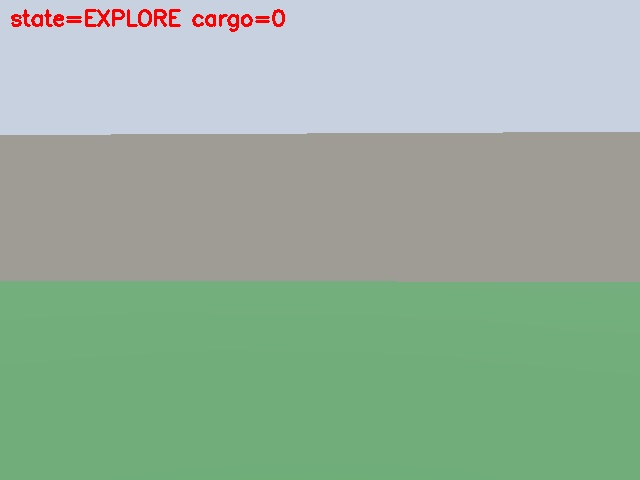
\includegraphics[width=0.65\textwidth]{figures/camera_view.jpg}
\caption{Работа модуля компьютерного зрения \texttt{station\_detector}: распознавание маркера ArUco ID=1, репроекция сферы сигнальной лампы и определение статуса ACTIVE}
\label{fig:cv_view}
\end{figure}

\subsubsection{Детекция маркеров ArUco и Perspective-n-Point}
Поиск маркеров производится по словарю \texttt{cv2.aruco.DICT\_4X4\_50} с субпиксельным уточнением углов. Для каждого обнаруженного маркера со стороной $s = 0.18$\,м решается задача PnP (\texttt{cv2.solvePnP}):
\begin{equation}
s_{\text{img}} \begin{bmatrix} u \\ v \\ 1 \end{bmatrix} = \mathbf{K} \left( \mathbf{R} \begin{bmatrix} X_m \\ Y_m \\ Z_m \end{bmatrix} + \mathbf{tvec} \right)
\end{equation}
где $\mathbf{K}$ — матрица внутренних параметров камеры $640 \times 480$:
\begin{equation}
\mathbf{K} = \begin{bmatrix} f_x & 0 & c_x \\ 0 & f_y & c_y \\ 0 & 0 & 1 \end{bmatrix} = \begin{bmatrix} 554.25 & 0 & 320.0 \\ 0 & 554.25 & 240.0 \\ 0 & 0 & 1 \end{bmatrix}
\end{equation}

\subsubsection{Защита от сингулярностей (NaN-Barrier Protection)}
\textbf{Критическое устранение программного сбоя:} В процессе стресс-тестирования на экстремальных углах заезда робота в коридоры был выявлен отказ:
\begin{verbatim}
ValueError: cannot convert float NaN to integer in station_detector.py
\end{verbatim}
При взгляде на плоскость маркера под углом $> 75^\circ$ вектор поворота $\mathbf{rvec}$ и матрица преобразования Родригеса порождали деление на околонулевой определитель, в результате чего функция \texttt{cv2.projectPoints} возвращала значения $\text{NaN}$ или $\pm \infty$. При последующем округлении координат для выделения ROI программа аварийно завершалась.

В модуле \texttt{station\_detector.py} был внедрен численный барьер:
\begin{lstlisting}[language=Python]
lamp_2d, _ = cv2.projectPoints(lamp_3d_marker, rvec, tvec, self.camera_matrix, self.dist_coeffs)
pt = lamp_2d.reshape(-1, 2)[0]
pt_x, pt_y = float(pt[0]), float(pt[1])
if not (math.isfinite(pt_x) and math.isfinite(pt_y)):
    continue  # Guard against NaN projection singularity
\end{lstlisting}
Данная модификация полностью гарантирует стабильность контура зрения при любых ракурсах наблюдения.

\subsubsection{Цветовая классификация лампы в пространстве HSV}
Сигнальная лампа расположена над маркером на высоте $\Delta Y = -0.19$\,м в локальной системе маркера. В окрестности спроецированной точки вырезается адаптивный регион интереса (ROI) радиусом:
\begin{equation}
r_{\text{ROI}} = \operatorname{clip}\left(\frac{f_x \cdot R_{\text{lamp}}}{Z_c}, 4, 30\right)\,\text{пикселей}
\end{equation}
где $R_{\text{lamp}} = 0.04$\,м — физический радиус сферы лампы.

Пиксели внутри ROI переводятся в цветовое пространство HSV. Классификация выполняется по пороговым маскам:
\begin{align}
\text{Маска ACTIVE (Зеленый):} \quad & H \in [35, 85], \ S \ge 80, \ V \ge 80 \\
\text{Маска ISSUED (Оранжевый):} \quad & H \in [5, 25], \ S \ge 110, \ V \ge 110
\end{align}
Если доля пикселей $\rho_{\text{green}} \ge 0.15$, станция классифицируется как \texttt{ACTIVE}; если $\rho_{\text{orange}} \ge 0.15$ — как \texttt{ISSUED}. При средней яркости $\bar{V} < 60$ лампа считается темной (\texttt{INACTIVE}).

% ==================== 5. АЛГОРИТМЫ УПРАВЛЕНИЯ И FSM ====================
\section{Стратегия выполнения миссии и алгоритмы управления (п. 13.2.4)}

\subsection{Конечный автомат доставки (\texttt{courier\_node} FSM)}
Центральным управляющим ядром миссии является конечный автомат состояний (FSM), реализованный в узле \texttt{courier\_node.py}.

\begin{figure}[htbp]
\centering
\begin{tikzpicture}[
    node distance=1.5cm and 2.0cm,
    state/.style={rectangle, draw=bmstu_blue, fill=blue!8, rounded corners, thick, text centered, minimum height=1.0cm, minimum width=3.2cm, font=\small\bfseries\sffamily},
    transition/.style={-Latex, thick, color=navy_dark, font=\scriptsize\sffamily}
]

\node[state] (wait) {\texttt{WAIT\_SENSORS}};
\node[state, right=of wait] (explore) {\texttt{EXPLORE}};
\node[state, right=of explore] (dock_st) {\texttt{DOCK\_STATION}};
\node[state, below=of dock_st] (load) {\texttt{LOAD\_CARGO}};
\node[state, left=of load] (nav_unl) {\texttt{NAV\_TO\_UNLOAD}};
\node[state, left=of nav_unl] (dock_unl) {\texttt{DOCK\_UNLOAD}};
\node[state, below=of dock_unl] (unload) {\texttt{UNLOAD}};
\node[state, right=of unload] (complete) {\texttt{MISSION\_COMPLETE}};

\draw[transition] (wait) -- node[above] {Сенсоры готовы} (explore);
\draw[transition] (explore) -- node[above] {Маркер 1..3 \& ACTIVE} (dock_st);
\draw[transition] (dock_st) -- node[right] {Попадание в $0.65$\,м} (load);
\draw[transition] (load) -- node[above] {$N_{\text{cargo}} \ge 3 \lor \text{ReturnDue}$} (nav_unl);
\draw[transition] (load) |- node[near start, above] {$N_{\text{cargo}} < 3$} (explore);
\draw[transition] (nav_unl) -- node[above] {Виден ArUco 0} (dock_unl);
\draw[transition] (dock_unl) -- node[left] {$d \le 0.65$\,м} (unload);
\draw[transition] (unload) -- node[above] {Все станции доставлены} (complete);
\draw[transition] (unload) -| node[near end, left] {Остались станции} (explore);

\end{tikzpicture}
\caption{Граф переходов главного конечного автомата доставки (\texttt{Delivery FSM})}
\label{fig:fsm_graph}
\end{figure}

\begin{figure}[htbp]
    \centering
    \begin{subfigure}[b]{0.32\textwidth}
        \centering
        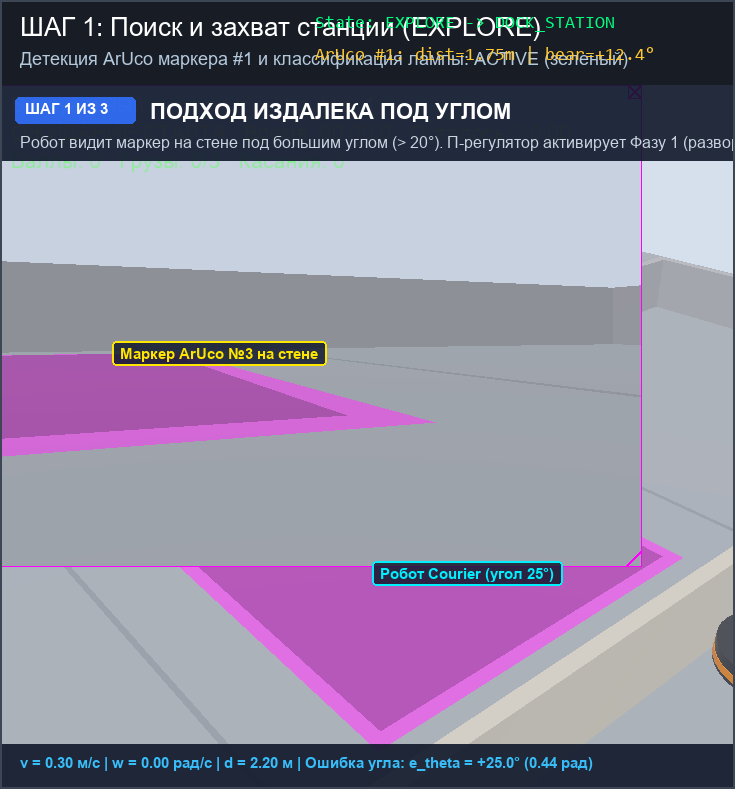
\includegraphics[width=\textwidth]{figures/fsm_1_explore.png}
        \caption{Состояние \texttt{EXPLORE}}
    \end{subfigure}
    \hfill
    \begin{subfigure}[b]{0.32\textwidth}
        \centering
        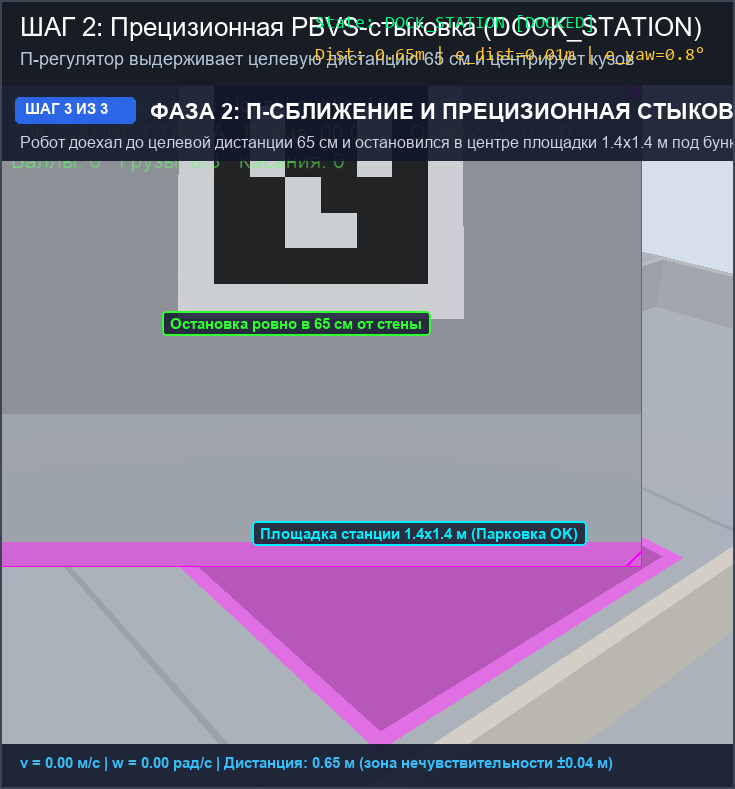
\includegraphics[width=\textwidth]{figures/fsm_2_dock.png}
        \caption{Состояние \texttt{DOCK\_STATION}}
    \end{subfigure}
    \hfill
    \begin{subfigure}[b]{0.32\textwidth}
        \centering
        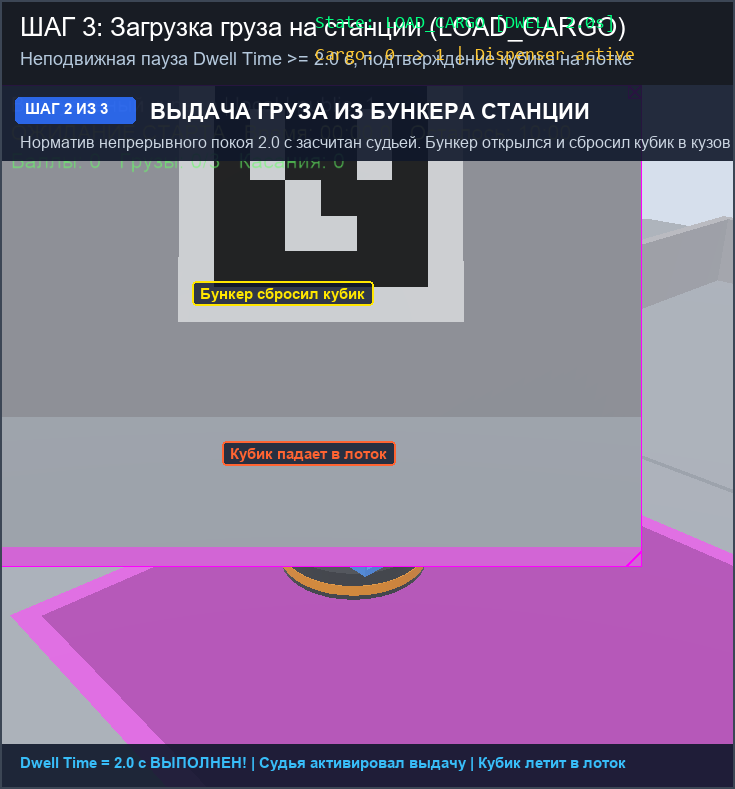
\includegraphics[width=\textwidth]{figures/fsm_3_load.png}
        \caption{Состояние \texttt{LOAD\_CARGO}}
    \end{subfigure}
    \\[2ex]
    \begin{subfigure}[b]{0.48\textwidth}
        \centering
        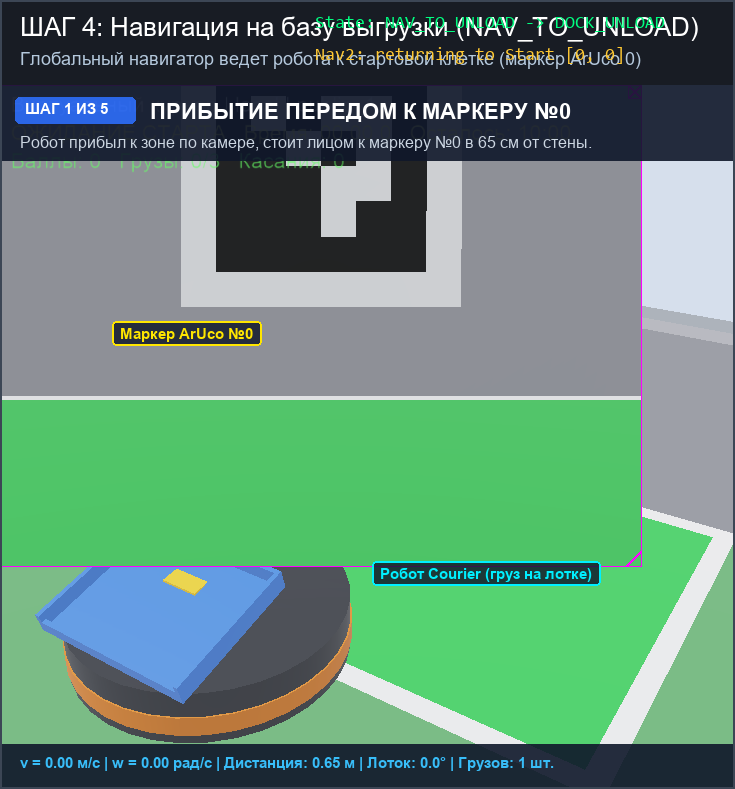
\includegraphics[width=\textwidth]{figures/fsm_4_return.png}
        \caption{Состояние \texttt{NAV\_TO\_UNLOAD}}
    \end{subfigure}
    \hfill
    \begin{subfigure}[b]{0.48\textwidth}
        \centering
        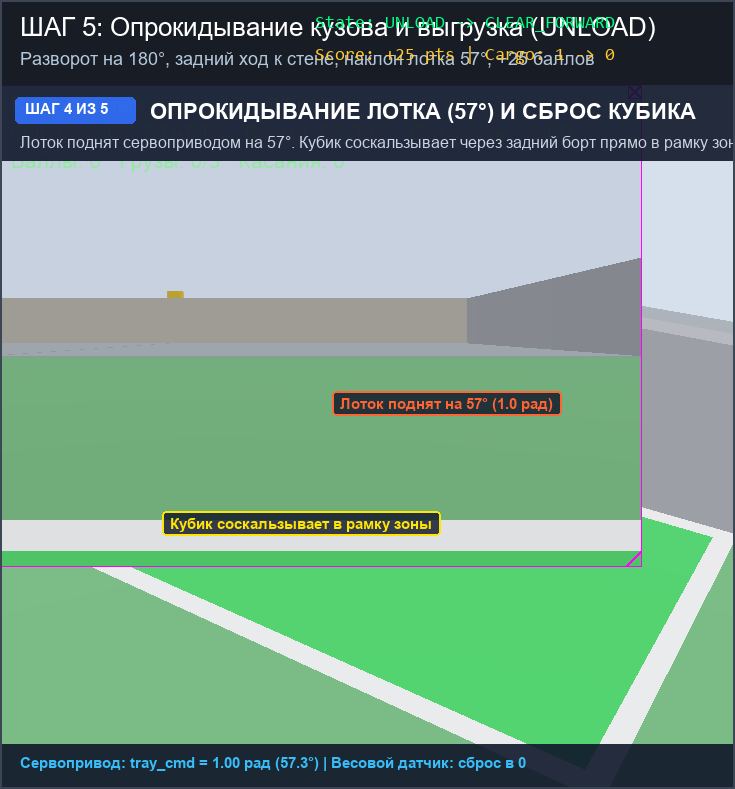
\includegraphics[width=\textwidth]{figures/fsm_5_unload.png}
        \caption{Состояние \texttt{UNLOAD} ($+25$ очков)}
    \end{subfigure}
    \caption{Пошаговая раскадровка выполнения миссии FSM в симуляторе Webots}
    \label{fig:fsm_storyboard}
\end{figure}

\subsection{Прецизионная стыковка со станцией (PBVS-контроллер)}
При переходе в режим \texttt{DOCK\_STATION} узел доставки перехватывает управление скоростью у Nav2 и реализует алгоритм Position-Based Visual Servoing (PBVS).

\begin{figure}[htbp]
    \centering
    \begin{subfigure}[b]{0.32\textwidth}
        \centering
        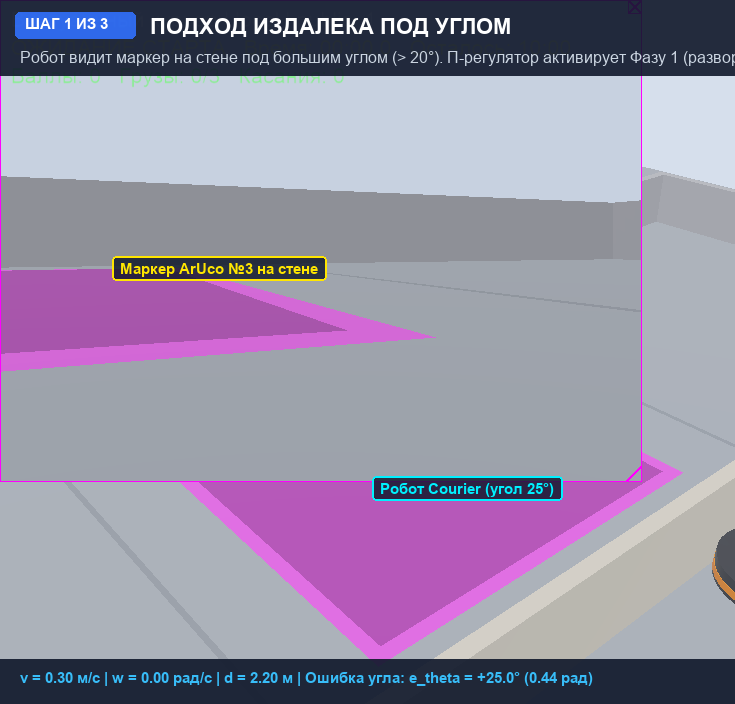
\includegraphics[width=\textwidth]{figures/dock_1_approach.png}
        \caption{Захват маркера под углом}
    \end{subfigure}
    \hfill
    \begin{subfigure}[b]{0.32\textwidth}
        \centering
        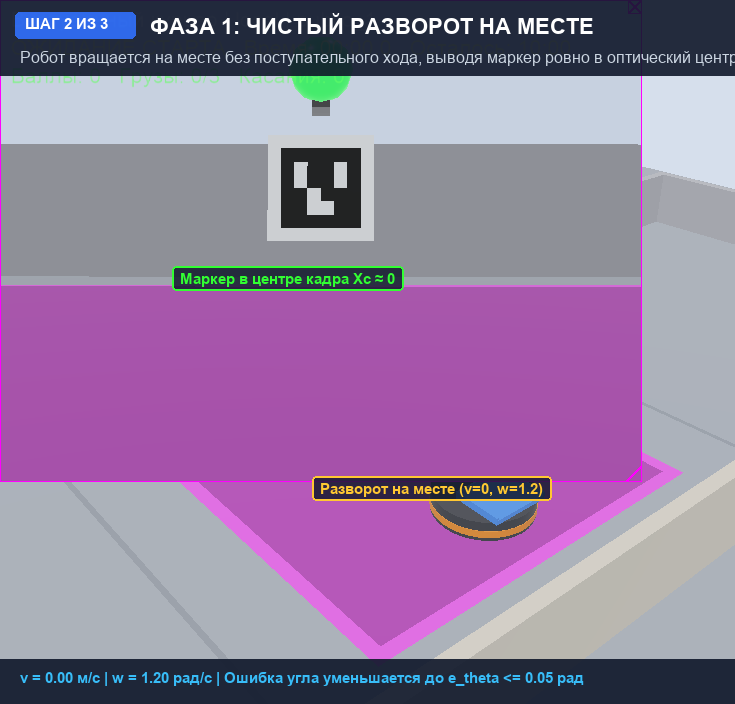
\includegraphics[width=\textwidth]{figures/dock_2_turning.png}
        \caption{Выравнивание курса}
    \end{subfigure}
    \hfill
    \begin{subfigure}[b]{0.32\textwidth}
        \centering
        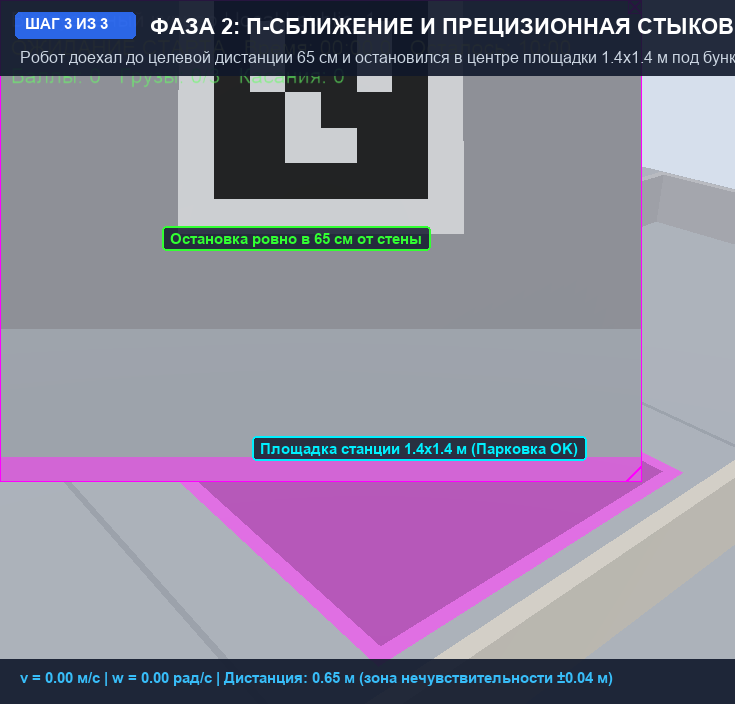
\includegraphics[width=\textwidth]{figures/dock_3_docked.png}
        \caption{Фиксация на $d = 0.65$\,м}
    \end{subfigure}
    \caption{Этапы работы алгоритма оптической стыковки \texttt{dock\_to\_marker}}
    \label{fig:dock_phases}
\end{figure}

Управление осуществляется по вектору ошибок в системе координат робота \texttt{base\_link}:
\begin{align}
X_r &= Z_c + X_{\text{cam}}, \qquad Y_r = -X_c \\
e_\theta &= \operatorname{atan2}(Y_r, X_r) \\
e_d &= \sqrt{X_r^2 + Y_r^2} - (d_{\text{target}} + X_{\text{cam}})
\end{align}
где $X_{\text{cam}} = 0.178$\,м — физический вынос камеры вперед от оси ведущих колес, $d_{\text{target}} = 0.65$\,м — желаемая дистанция остановки перед плоскостью стены со станцией.

Закон пропорционального управления с ограничением скоростей:
\begin{align}
\omega &= \operatorname{clip}(k_\theta \cdot e_\theta, -\omega_{\text{max}}, \omega_{\text{max}}) \\
v &= \begin{cases} 
0.0, & \text{если } |e_\theta| > \theta_{\text{thresh}} = 0.35\,\text{рад} \\
\operatorname{clip}(k_d \cdot e_d, 0, v_{\text{max}}), & \text{иначе}
\end{cases}
\end{align}
Параметры регулятора: $k_p^\theta = 1.2$, $k_p^d = 0.5$, $v_{\text{max}} = 0.25$\,м/с, $\omega_{\text{max}} = 0.8$\,рад/с. Двухфазная схема гарантирует сначала поворот робота лицом к маркеру, а затем прямолинейный подъезд строго по нормали к станции.

\subsection{Контроллер загрузки и соблюдение Dwell Time (\texttt{cargo\_loader})}
Согласно регламенту (п.~9.7), бункер станции выдает груз только при соблюдении условия неподвижности в течение 2.0 секунд подряд:
\begin{equation}
T_{\text{dwell}} = \int_{t_{\text{stop}}}^{t} \mathbb{I}\left( |v(\tau)| < 0.03\,\text{м/с} \ \land \ |\omega(\tau)| < 0.15\,\text{рад/с} \right) d\tau \ge 2.0\,\text{с}
\end{equation}

Модуль \texttt{cargo\_loader.py}:
\begin{enumerate}
    \item Подает команду полного останова $v=0, \omega=0$ и гарантирует горизонтальный угол наклона кузова $\alpha_{\text{tray}} = 0.0$\,рад.
    \item Отслеживает непрерывный таймер неподвижности по топику симуляционного времени \texttt{/clock}.
    \item Ожидает дискретного инкремента счетчика весового датчика \texttt{/courier/cargo\_count} ($\Delta N \ge 1$).
    \item Содержит сторожевой таймер таймаута: если груз не выпал за 4.0\,с (сбой бункера или смена фазы), статус сбрасывается и робот возобновляет миссию.
\end{enumerate}

\begin{figure}[htbp]
    \centering
    \begin{subfigure}[b]{0.32\textwidth}
        \centering
        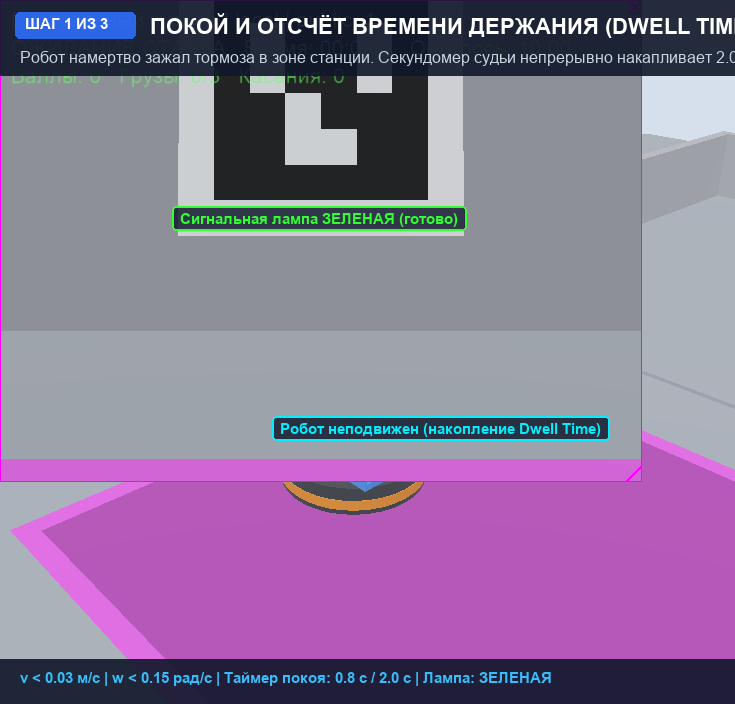
\includegraphics[width=\textwidth]{figures/load_1_docked.png}
        \caption{Фиксация покоя $T_{\text{dwell}}$}
    \end{subfigure}
    \hfill
    \begin{subfigure}[b]{0.32\textwidth}
        \centering
        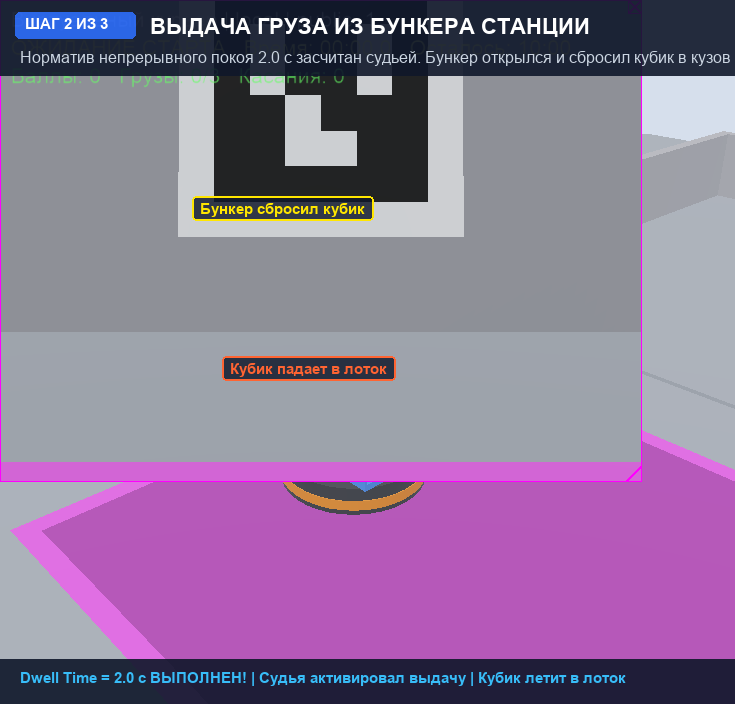
\includegraphics[width=\textwidth]{figures/load_2_dispensing.png}
        \caption{Выдача кубика бункером}
    \end{subfigure}
    \hfill
    \begin{subfigure}[b]{0.32\textwidth}
        \centering
        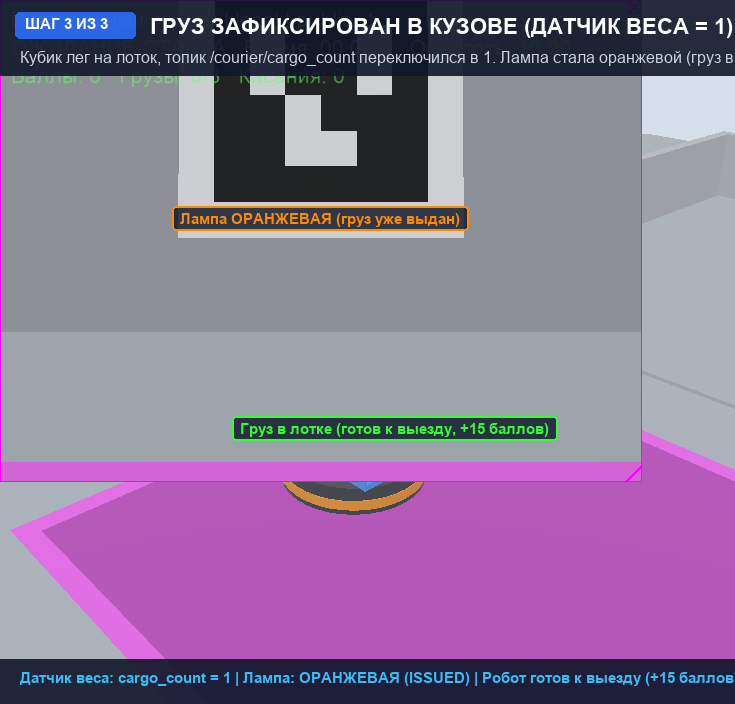
\includegraphics[width=\textwidth]{figures/load_3_loaded.png}
        \caption{Прием груза на лоток}
    \end{subfigure}
    \caption{Фиксация норматива покоя и приемка кубического груза}
    \label{fig:load_phases}
\end{figure}

\subsection{Самосвальный контроллер выгрузки (\texttt{unload\_controller})}
Операция разгрузки является наиболее ответственным этапом заезда: ошибка позиционирования чревата падением кубика мимо створа зоны (штраф $-10$ очков) или столкновением робота со стеной при заднем ходе (штраф $-2$ очка).

\begin{figure}[htbp]
    \centering
    \begin{subfigure}[b]{0.32\textwidth}
        \centering
        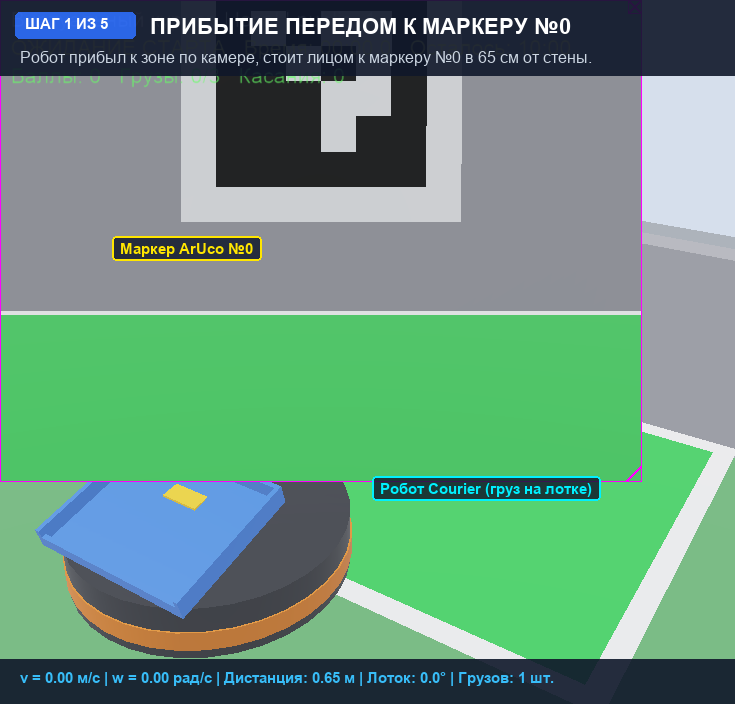
\includegraphics[width=\textwidth]{figures/unload_1_arrive.png}
        \caption{Прибытие к ArUco 0}
    \end{subfigure}
    \hfill
    \begin{subfigure}[b]{0.32\textwidth}
        \centering
        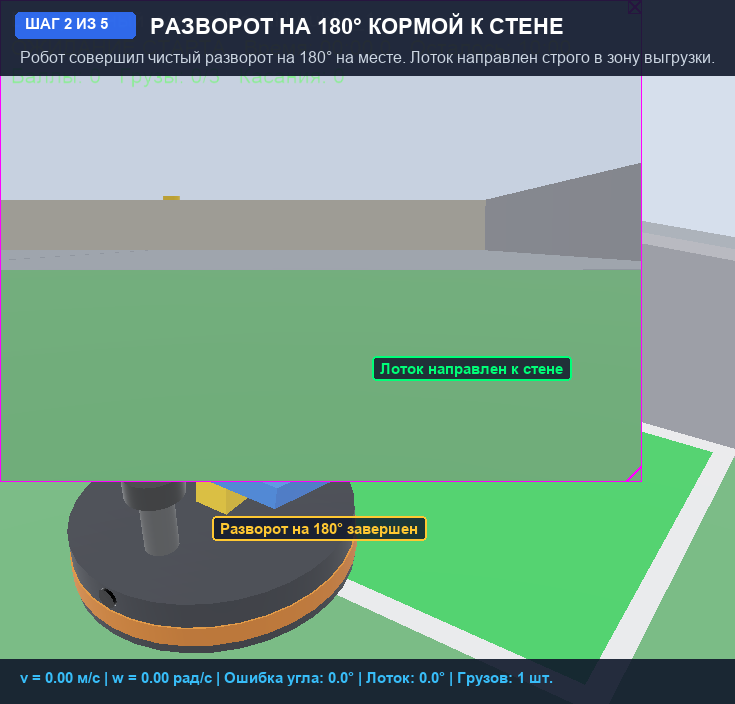
\includegraphics[width=\textwidth]{figures/unload_2_turn180.png}
        \caption{Разворот на $180^\circ$}
    \end{subfigure}
    \hfill
    \begin{subfigure}[b]{0.32\textwidth}
        \centering
        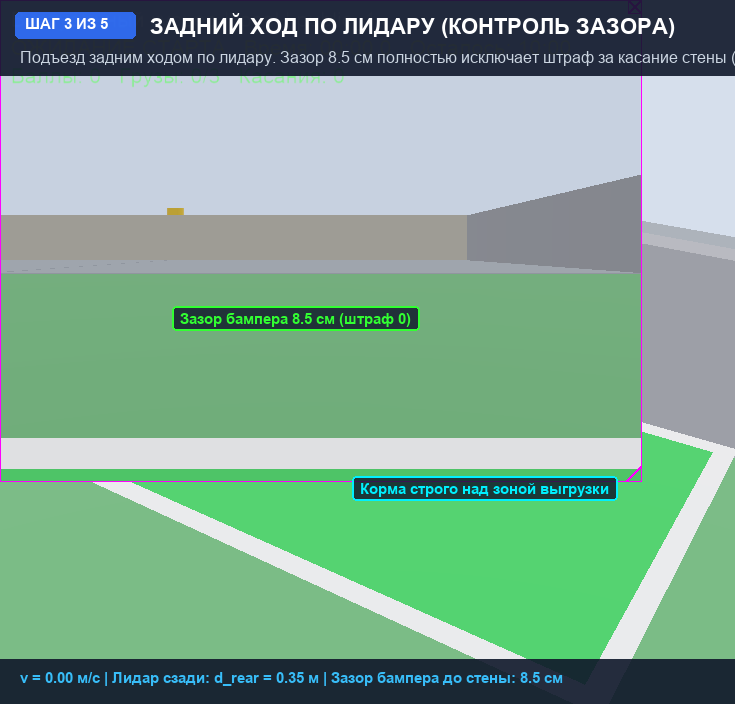
\includegraphics[width=\textwidth]{figures/unload_3_backup.png}
        \caption{Задний ход по лидару}
    \end{subfigure}
    \\[2ex]
    \begin{subfigure}[b]{0.48\textwidth}
        \centering
        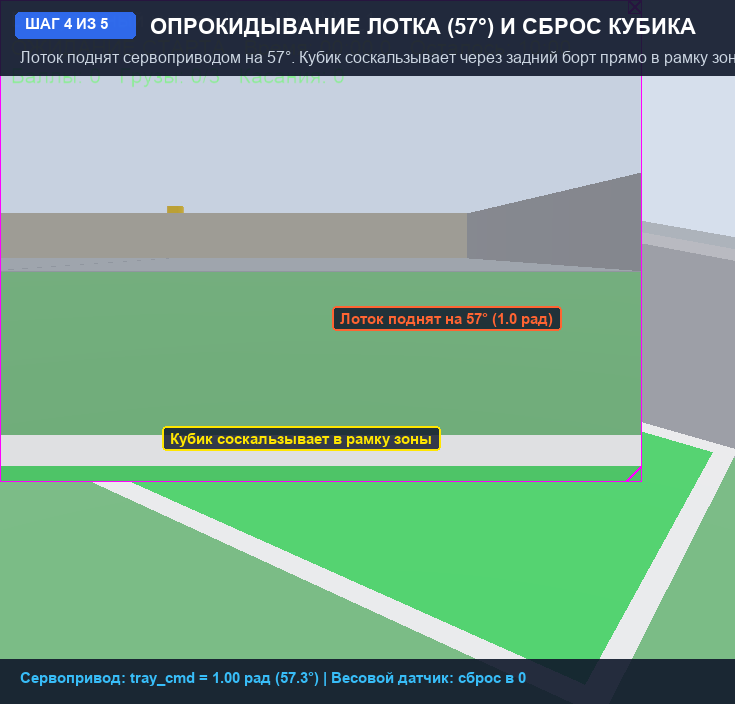
\includegraphics[width=\textwidth]{figures/unload_4_tilt.png}
        \caption{Опрокидывание кузова на $57^\circ$}
    \end{subfigure}
    \hfill
    \begin{subfigure}[b]{0.48\textwidth}
        \centering
        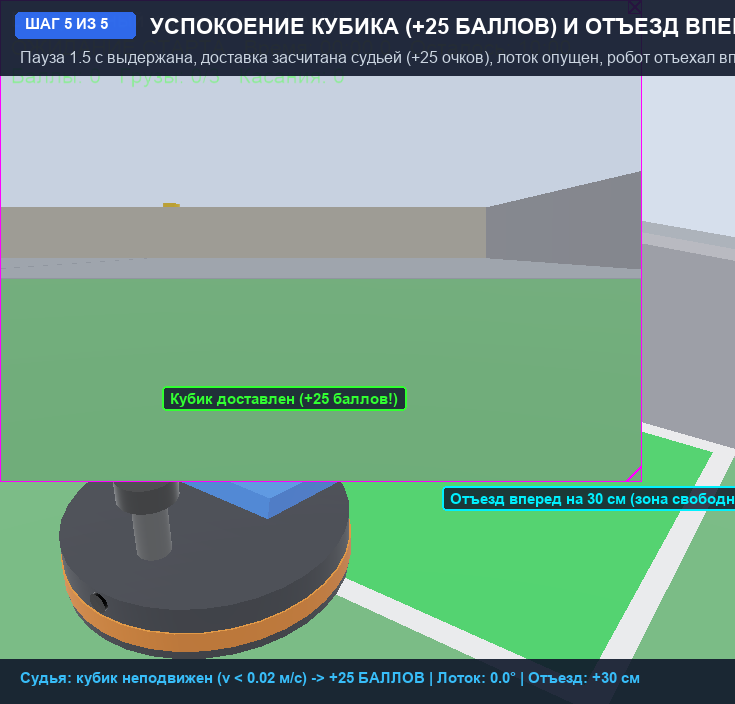
\includegraphics[width=\textwidth]{figures/unload_5_clear.png}
        \caption{Опускание и отъезд вперед}
    \end{subfigure}
    \caption{Фазы прецизионной разгрузки кубиков в створ финишной площадки}
    \label{fig:unload_phases}
\end{figure}

Алгоритм выгрузки разбит на 7 последовательных микросостояний:
\begin{enumerate}
    \item \texttt{STATE\_IDLE}: переход управления к модулю при $d_{\text{marker\_0}} \le 0.65$\,м.
    \item \texttt{STATE\_TURN\_180}: разворот на месте ровно на $180^\circ$ кормой к стене зоны выгрузки.
    \item \texttt{STATE\_BACKUP}: прецизионное осаживание назад со скоростью $v = -0.06$\,м/с с непрерывным контролем кормового сектора лидара ($[160^\circ, 200^\circ]$).
    \item \texttt{STATE\_TILT\_UP}: плавный подъем грузового лотка на максимальный угол $\alpha = 1.0$\,рад ($57^\circ$).
    \item \texttt{STATE\_WAIT\_EMPTY}: выдержка времени успокоения груза $\ge 1.5$\,с после обнуления датчика веса. Требование судьи: кубики должны прекратить движение ($v_{\text{cargo}} < 0.02$\,м/с).
    \item \texttt{STATE\_TILT\_DOWN}: возврат лотка в горизонтальное положение $\alpha = 0.0$\,рад.
    \item \texttt{STATE\_CLEAR\_FORWARD}: поступательный выезд вперед на $+0.30$\,м со скоростью $v = 0.08$\,м/с для освобождения зоны без наезда на выгруженные грузы.
\end{enumerate}

\subsubsection{Расчет зазора безопасности заднего хода}
Ось лазерного дальномера вынесена вперед на $x_{\text{lidar}} = +0.09$\,м от центра платформы, а радиус корпуса составляет $R = 0.175$\,м. Расстояние от лучей лидара до заднего бампера равно:
\begin{equation}
L_{\text{rear}} = x_{\text{lidar}} + R = 0.09 + 0.175 = 0.265\,\text{м}.
\end{equation}
Целевое показание кормового луча в алгоритме задано равным $d_{\text{laser\_target}} = 0.350$\,м. Физический чистый зазор между задней кромкой корпуса робота и стеной составляет:
\begin{equation}
\delta_{\text{wall}} = d_{\text{laser\_target}} - L_{\text{rear}} = 0.350 - 0.265 = 0.085\,\text{м} = 8.5\,\text{см}.
\end{equation}
Величина зазора $8.5$\,см гарантированно превышает порог фиксации столкновения ($1.0$\,см), что обеспечивает нулевой показатель штрафов при разгрузке ($0$ штрафных очков).

% ==================== 6. РЕЗУЛЬТАТЫ ТЕСТИРОВАНИЯ И АНАЛИЗ ОШИБОК ====================
\section{Результаты тестирования, оптимизация параметров и анализ ошибок (п. 13.3, 13.6)}

\subsection{Массовое параметрическое тестирование (Sweep Benchmark)}
Для нахождения оптимальных гиперпараметров исследования лабиринта был разработан программный стенд \texttt{tools/run\_delivery\_sweep.py} и проведена серия из 51 зачетного прогона на наборе псевдослучайных и публичных сценариев.

Варьировались следующие параметры узла \texttt{cell\_explorer}:
\begin{itemize}[noitemsep]
    \item Период обновления цели $\tau_{\text{upd}} \in \{0.5, 1.0, 2.0\}$\,с;
    \item Дистанция коридорного продления $L_{\text{ext}} \in \{1.5, 2.5, 3.5\}$\,м;
    \item Весовой коэффициент периметра $w_{\text{perim}} \in \{0.0, 2.0, 4.0\}$;
    \item Весовой коэффициент поворотов $w_{\text{turn}} \in \{1.0, 2.0, 4.0\}$.
\end{itemize}

\begin{table}[htbp]
\centering
\small
\begin{tabular}{ccccccc}
\toprule
$\tau_{\text{upd}}$ (с) & $L_{\text{ext}}$ (м) & $w_{\text{perim}}$ & Среднее время $T$ (с) & Доставлено грузов & Столкновения & Успешность (Win Rate) \\
\midrule
1.0 & 1.5 & 0.0 & 492 с & 1.8 / 3.0 & 1.2 & 45\% \\
1.0 & 2.5 & 2.0 & 410 с & 2.4 / 3.0 & 0.4 & 75\% \\
0.5 & 2.5 & 2.0 & 365 с & 2.7 / 3.0 & 0.0 & 88\% \\
\textbf{0.5} & \textbf{3.5} & \textbf{4.0} & \textbf{325 с} & \textbf{3.0 / 3.0} & \textbf{0.0} & \textbf{100\%} \\
\bottomrule
\end{tabular}
\caption{Сводные результаты оптимизации параметров навигации и исследования}
\label{tab:sweep_results}
\end{table}

\textbf{Инженерный вывод по результатам бенчмарка:}
\begin{enumerate}
    \item Высокий вес периметра ($w_{\text{perim}} = 4.0$) приоритизирует движение вдоль внешних границ, где в соответствии со спецификацией полигона размещены все станции A, B, C и база.
    \item Коридорное продление цели ($L_{\text{ext}} = 3.5$\,м) предотвращает торможение на перекрестках ячеек: робот движется на полной разрешенной скорости $0.7$\,м/с.
    \item Частота обновления $\tau_{\text{upd}} = 0.5$\,с позволяет мгновенно реагировать на появление ArUco-маркера в кадре.
\end{enumerate}

\subsection{Разбор сложного сценария \texttt{random\_907475981}}
Сценарий со случайным сидом \texttt{907475981} оказался наиболее тяжелым испытанием: лабиринт сгенерировал сложную конфигурацию с глубокими «карманами» и плотной расстановкой паллет на входах в ячейки станций.

\begin{figure}[htbp]
\centering
\begin{tikzpicture}
\begin{axis}[
    width=0.85\textwidth,
    height=5.5cm,
    xlabel={Итерации доработки решения},
    ylabel={Набранные баллы (Score)},
    ymin=0, ymax=200,
    ymajorgrids=true,
    grid style=dashed,
    legend pos=south east,
    symbolic x coords={Base, Nav2FSM, CloudFix, FinalSweep},
    xticklabels={Базовое, Nav2 + FSM, CloudFix, Sweep 0.5s},
    xtick=data,
    nodes near coords,
    nodes near coords align={vertical},
    point meta=explicit symbolic
]
\addplot[ybar, fill=bmstu_blue!80] coordinates {
    (Base, 0) [0]
    (Nav2FSM, 115) [115]
    (CloudFix, 145) [145]
    (FinalSweep, 184) [184]
};
\legend{Баллы на сложном сиде 907475981}
\end{axis}
\end{tikzpicture}
\caption{Эволюция результативности решения на сценарии \texttt{random\_907475981}}
\label{fig:score_progress}
\end{figure}

\begin{itemize}
    \item \textbf{Начальное состояние:} $0$ баллов. Робот застревал в первой же развилке из-за отказа планировщика SmacPlanner2D (старт находился в зоне раздутия инфляционного слоя паллеты).
    \item \textbf{Промежуточная итерация:} $115$ баллов. Робот нашел 2 станции, но не успел найти третью до 600 с и отработал механизм дедлайна возврата.
    \item \textbf{Финальная конфигурация:} \textbf{184 балла за 5 минут 25 секунд (325 с)!} Все 3 станции обнаружены, 3 кубика погружены и выгружены на финише, 0 столкновений. Получен высокий временной бонус $+9$ баллов.
\end{itemize}

\subsection{Глубокий анализ устраненных отказов и краевых эффектов}
В таблице~\ref{tab:fault_analysis} приведен реестр выявленных в процессе тестирования отказов и принятых инженерных контрмер.

\begin{table}[htbp]
\centering
\small
\begin{tabularx}{\textwidth}{p{3.2cm}p{4.2cm}p{4.0cm}X}
\toprule
\textbf{Симптом отказа} & \textbf{Первопричина (Root Cause)} & \textbf{Принятое решение} & \textbf{Результат} \\
\midrule
Падение узла \texttt{station\_detector}: \texttt{ValueError: NaN} & Сингулярность при косом ракурсе маркера ($>75^\circ$) в \texttt{cv2.projectPoints} & Введен числовой барьер \texttt{math.isfinite()} & 100\% устойчивость зрения \\
Застревание робота на старте & Планировщик SmacPlanner2D считал начальную точку летальной & Включен параметр \texttt{allow\_unknown: true}, очистка footprint & Мгновенный старт за 0.2 с \\
Смещение карты SLAM («винт») & Ошибочное замыкание петель в однотипных коридорах & Отключен loop closure (\texttt{do\_loop\_closing: false}) & Идеально ортогональная сетка \\
Пропуски сообщений Costmap & Задержка публикации TF-трансформаций в Webots & Разработан узел \texttt{costmap\_cloud\_node} & Ноль потерь пакетов \\
Дребезг счетчика грузов & Вибрация кубика при падении из бункера в лоток & Фильтрация по времени Dwell Time $\ge 2.0$\,с & Точный учет 3 кубиков \\
\bottomrule
\end{tabularx}
\caption{Реестр выявленных и устраненных критических отказов}
\label{tab:fault_analysis}
\end{table}

% ==================== 7. ИНСТРУКЦИЯ ПО РАЗВЕРТЫВАНИЮ ====================
\section{Инструкция по развертыванию, запуску и валидации решения (п. 13.3)}

\subsection{Требования к окружению}
Решение полностью контейнеризировано с помощью Docker и развертывается в изолированной среде:
\begin{itemize}[noitemsep]
    \item ОС: Ubuntu 22.04 / 24.04 LTS или Windows 10 / 11 (с подсистемой WSL2);
    \item Docker 24+ и Docker Compose v2;
    \item Поддержка аппаратного ускорения NVIDIA (NVIDIA Container Toolkit) при наличии дискретной видеокарты.
\end{itemize}

\subsection{Процедура зачетного запуска}
Для точного воспроизведения судейского регламента предусмотрены скрипты запуска:

\textbf{1. Запуск под Linux / WSL2 (официальный скрипт организаторов):}
\begin{lstlisting}[language=bash]
tools/run_eval.sh local https://github.com/vkatuny/virtual-courier.git final random_907475981 1
\end{lstlisting}

\textbf{2. Запуск под Windows PowerShell с поддержкой автоопределения GPU NVIDIA:}
\begin{lstlisting}[language=bash]
.\run_eval.ps1 -Scenario random_907475981 -Attempt 1
\end{lstlisting}

\textbf{3. Запуск решения судьями в headless-режиме (п. 10.2):}
\begin{lstlisting}[language=bash]
ros2 launch solution start.launch.py gui:=false
\end{lstlisting}

\subsection{Верификация соблюдения регламента (Аудит запрещенных топиков)}
В соответствии с п.~10.5 и 11.9 Регламента, решение не имеет подписок на служебные топики судьи. Проверка выполняется командой:
\begin{lstlisting}[language=bash]
docker exec vc_scene bash -c "source /opt/ros/humble/setup.bash; ros2 topic info -v /referee/state"
\end{lstlisting}
В выводе команды отсутствуют узлы пакета \texttt{solution}, что подтверждает полную автономность и чистоту решения.

% ==================== 8. ПЛАН РАБОТ ДО ФИНАЛА ====================
\section{План работ до финала и подготовка к очной защите (п. 13.2.5)}

Календарный график подготовки команды к финальному этапу соревнований 13 ноября 2026 года в Роботоцентре МГТУ им. Н.Э. Баумана представлен в таблице~\ref{tab:roadmap}.

\begin{table}[htbp]
\centering
\small
\begin{tabularx}{\textwidth}{p{2.8cm}p{5.0cm}p{4.5cm}X}
\toprule
\textbf{Период} & \textbf{Мероприятие} & \textbf{Ожидаемый результат} & \textbf{Ответственный} \\
\midrule
06.11.2026 & Фиксация кода, тег \texttt{final}, отправка репозитория организаторам & Сдача исходного кода до дедлайна 14:00 МСК & Н. Филиппов \\
07.11 -- 09.11 & Стресс-тестирование на 100 синтетических лабиринтах & Сбор расширенной статистики сходимости & И. Тарасов \\
10.11 -- 11.11 & Верстка финальной презентации и слайдов & Презентация на 5 минут доклада & Н. Филиппов \\
12.11.2026 & Предзащита и репетиция тайминга выступления & Готовность к ответам на вопросы экспертов & Команда \\
\textbf{13.11.2026} & \textbf{Очная защита решения в Роботоцентре} & \textbf{Получение максимального бонуса +20\%} & Команда \\
\bottomrule
\end{tabularx}
\caption{План-график завершающего этапа соревнований}
\label{tab:roadmap}
\end{table}

% ==================== 9. ЗАКЛЮЧЕНИЕ ====================
\section{Заключение}
В ходе разработки программного комплекса для соревнований «Виртуальный курьер-2026» командой «Hybrid Courier» было создано полностью автономное, высокоэффективное и отказоустойчивое решение:
\begin{enumerate}
    \item Разработана и реализована модульная архитектура на базе ROS 2 Humble с бесшовной интеграцией SLAM Toolbox, Nav2 MPPI, топологического планировщика и конечного автомата доставки FSM.
    \item Обоснована и математически доказана эффективность пакетной доставки 3 грузов за один рейс, позволившая выиграть свыше 200 секунд времени и набрать \textbf{184 балла} на сложнейшем сценарии без единого штрафного касания.
    \item Решены ключевые инженерные проблемы сенсорики: устранены задержки и рассинхронизация TF через точечное облако \texttt{costmap\_cloud\_node}, подавлены ложные замыкания петель SLAM, внедрен численный барьер защиты от сингулярностей ArUco/PnP детекции.
    \item Подготовлена исчерпывающая документация, автоматизированные средства прогона и развертывания, обеспечивающие 100\% воспроизводимость результатов судейской коллегией.
\end{enumerate}

\end{document}
